% PNP (Purine Nucleoside Phosphorylase) Reaction Diagram
% MESG + Pi -> 7-Methyl-6-thioguanine + alpha-D-ribose-1-phosphate
% Matches original diagram layout: vertical flow, molecular structures
% with colored atoms, PNP arrow in center, Absorbance 360nm at bottom
%
% Color coding:
%   blue   = nitrogen (N)
%   red    = oxygen (O)
%   yellow = sulfur (S)
%   orange = phosphorus (P)
%
% Compile:  pdflatex -output-directory=molecular_diagrams molecular_diagrams/pnp_reaction.tex

\documentclass[border=10pt]{standalone}
\usepackage[utf8]{inputenc}
\usepackage{chemfig}
\usepackage{xcolor}
\usepackage{amsmath}
\usepackage{array}
\usepackage{tikz}

% ---- Colour definitions ---------------------------------------------------
\definecolor{Ncolor}{HTML}{0066CC}
\definecolor{Ocolor}{HTML}{CC0000}
\definecolor{Scolor}{HTML}{D4A017}
\definecolor{Pcolor}{HTML}{E07000}

% ---- Helper macros for coloured atoms in chemfig --------------------------
\newcommand{\Natom}{\textcolor{Ncolor}{N}}
\newcommand{\Oatom}{\textcolor{Ocolor}{O}}
\newcommand{\Satom}{\textcolor{Scolor}{S}}
\newcommand{\Patom}{\textcolor{Pcolor}{P}}

\begin{document}

\begin{tabular}{c}

% ============================================================
% TOP: Reactants — MESG + Pi (side by side)
% ============================================================

\begin{tabular}{cc}

% --- MESG (7-Methyl-6-thioguanosine) ---
% Purine base: pyrimidine ring fused to imidazole
% NH2 at C2, S at C6, CH3 at N7, ribose at N9
\begin{tabular}{c}
\chemfig{
  % Pyrimidine ring (6-membered)
  *6(
    -=-(-NH_2)-
    % N3
    \Natom=
    % C4 - fusion point to imidazole
    (-[6]*5(
      -\Natom(-CH_3)=
      \Natom-
      % C8
      =-
    ))
    % C5 back to pyrimidine
    =
    % C6 with S (thione/thiol)
    (-\Satom)=
  )
  % N9 with ribose
  (-\Natom(-[1]
    % Ribose furanose ring
    [:-30]\Oatom-[7](-[1]OH)(-[7]OH)-[6](-[6]OH)-[5]
  ))
}

\\[4pt]
{\small\textbf{MESG}} \\
{\scriptsize 7-Methyl-6-thioguanosine}
\end{tabular}

&

% --- Pi (Inorganic phosphate) ---
\begin{tabular}{c}
\chemfig{\Patom(=[:90]\Oatom)(-[:-30]\Oatom^{-})(-[:150]\Oatom^{-})(-[:-90]OH)}

\\[4pt]
{\small\textbf{$P_i$}} \\
{\scriptsize Inorganic phosphate}
\end{tabular}

\end{tabular}

\\[1.5em]

% ============================================================
% MIDDLE: PNP enzyme arrow (vertical, downward)
% ============================================================

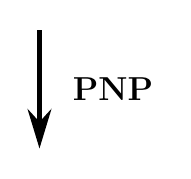
\begin{tikzpicture}
\draw[-{Stealth[length=5mm,width=3mm]},line width=2pt] (0,0) -- (0,-1.5);
\node[anchor=west] at (0.3,-0.75) {\large\bfseries PNP};
\end{tikzpicture}

\\[0.5em]

% ============================================================
% BOTTOM: Products — 7-Methyl-6-thioguanine + Ribose-1-phosphate
% ============================================================

\begin{tabular}{cc}

% --- 7-Methyl-6-thioguanine (free base, no ribose) ---
\begin{tabular}{c}
\chemfig{
  *6(
    -=-(-NH_2)-
    \Natom=
    (-[6]*5(
      -\Natom(-CH_3)=
      \Natom-
      =-
    ))
    =
    (-\Satom)=
  )
  % N9 with H instead of ribose
  (-\Natom(-[1]H))
}

\\[4pt]
{\small\textbf{7-Methyl-6-thioguanine}} \\
{\scriptsize 2-amino-6-mercapto-7-methylpurine}
\end{tabular}

&

% --- Ribose-1-phosphate ---
\begin{tabular}{c}
\chemfig{
  % Phosphate at C1
  \Oatom-[:30]\Patom(=[:90]\Oatom)(-[:-30]\Oatom^{-})(-[:150]OH)
  -[:-30]
  % Ribose furanose ring
  [:-30]\Oatom-[7](-[1]OH)(-[7]OH)-[6](-[6]OH)-[5]
}

\\[4pt]
{\small\textbf{Ribose-1-phosphate}} \\
{\scriptsize $\alpha$-D-ribofuranose-1-phosphate}
\end{tabular}

\end{tabular}

\\[1.5em]

% ============================================================
% BOTTOM LABEL: Detection method
% ============================================================

{\large\textit{Absorbance at 360\,nm}}

\end{tabular}

\end{document}